% !TeX root = ../main.tex

\chapter{LAMMPS 在申威平台上的并行实现}


\section{LAMMPS 计算平台介绍}
\subsection{LAMMPS 软件介绍}
LAMMPS(Large-scale Atomic/Molecular Massively Parallel Simulator)作为分子动力学计算领域内模拟体系涵盖最广的计算平台之一,由隶属于美国能源部的桑迪亚国家实验室进行开发和维护,可以进行多种体系的分子动力学模拟计算,包括生物大分子的结构微观模拟,合金等复合材料的热稳定性等机械性能。在材料力学中统计温度变化下势能,弹性常数的变化情况,并且提供了涉及多重体系的大量势函数,可以同时模拟出于固液气不同状态下的粒子行为,相比于其他分子动力学软件,例如GROMACS\cite{berendsen1995gromacs},NAMD\cite{phillips2005scalable},AMBER\cite{pearlman1995amber},CHARMM\cite{brooks1983charmm},拥有计算模型丰富,运行性能强大,上手容易等特点,软件代码迭代周期短,主要由 C++ 进行编写,其计算性能出色,已经在许多大型计算机上完成了不同体系下的多类大规模计算。针对并行计算的情况LAMMPS 采用了空间分解的方法将模拟体系划分为多个区域,并将子区域按需分配给不同的处理器进行计算。

LAMMPS 项目在20 世纪90 年代中期开始,直到2004 年给出了第一个开源版本,并且知道如今仍然以相当快的速度进行更新。截至 2021 年 4 月,最新的版本是8APR2021。LAMMPS 在提供大量势函数以及计算力场的基础上,同时也支持大量的硬件加速平台,并且针对这些平台额外编写了众多加速包进行支持,例如Nvidia GPU\cite{hong2009analytical},AMD ROCm\cite{kuznetsov2019porting},Intel CPU 以及Xeon phi\cite{chrysos2014intel}。在加速模块中也提供了许多并行方法可供参考,如CUDA,OpenCL,ROCm HIP,OpenMP, MPI 等。LAMMPS 本身也对通用 CPU 的多种向量化指令集提供了支持,包括SSE2\cite{bik2002automatic},AVX256\cite{lim2018implementation},AVX512\cite{cornea2015intel} 等。

\subsection{LAMMPS 工作流程介绍}
LAMMPS 的主要工作流程大致可分为三部分:初始化过程,模拟与计算,数据的后处理过程。

\subsubsection{初始化过程}
首先生成输入数据文件,这里可以根据计算模拟的体系与类型来控制数据文件,可以使用 matlab 进行数据文件的生成,其中包括体系中粒子的规模,类型个数,所分布区域的范围,然后为每个粒子设置相关参数,包括初始化位置坐标,自旋类型,编号及带电量等。接下来再编写输入配置文件,可以在配置文件中通过编写计算参数来模拟不同的计算过程,主要包括设置边界条件,时间步长,续算文件的控制,还可以描述输出结果的频率与所在模拟过程的系综。

\subsubsection{模拟与计算过程}
通过输入文件将体系中的粒子数据读入并形成完整的初始体系,首先利用Minimize 过程进行能量最小化的步骤,使其达到一个能够模拟稳定的初始状态,然后通过设置温度来为体系中所有粒子赋一个初速度,粒子开始无规则运动并进行一定时间步的弛豫过程,使粒子出于一个分散的状态,之后通过对体系边界的收缩产生激波使粒子随激波进行定向运动。在整个模拟过程中以牛顿定律为基础,通过对粒子间作用力的变化产生加速度与速度的改变,最后再把每个周期粒子信息记录下来,形成完整的运动轨迹。通过电子力场势函数完成对粒子间作用力的计算是最复杂也最耗时的部分,而在并行计算的过程中,通信的时间也占用了不小的比例。在完成每个时间步作用力的计算后,由于粒子的坐标位置不断变化,粒子对应的邻接表信息也会发生改变。过大的时间步长会使模拟的计算结果发散,所以这里选择△t = 0.005fs 作为整体计算的时间步长,而完成整个模拟计算则至少需要几十万的时间步。

\subsubsection{后处理过程}
在完成各个阶段的计算之后,LAMMPS 会给出多个不同类型的输出文件来对整个模拟过程进行量化的描述,以供后续的处理和分析。其中包括结果日志文件,结构文件,不同粒子的轨迹文件,续算文件等。再通过可视化工具对计算结果进行基本的分析处理,并验证结果的正确性。可视化工具包括OVITO,VMD等。这里能够获得在不同的模拟阶段不同类型粒子结构的运动轨迹和状态,最后通过 matlab 或 python 脚本完成粒子的多角度统计和分析。

 \begin{figure}[h]
  \centering
  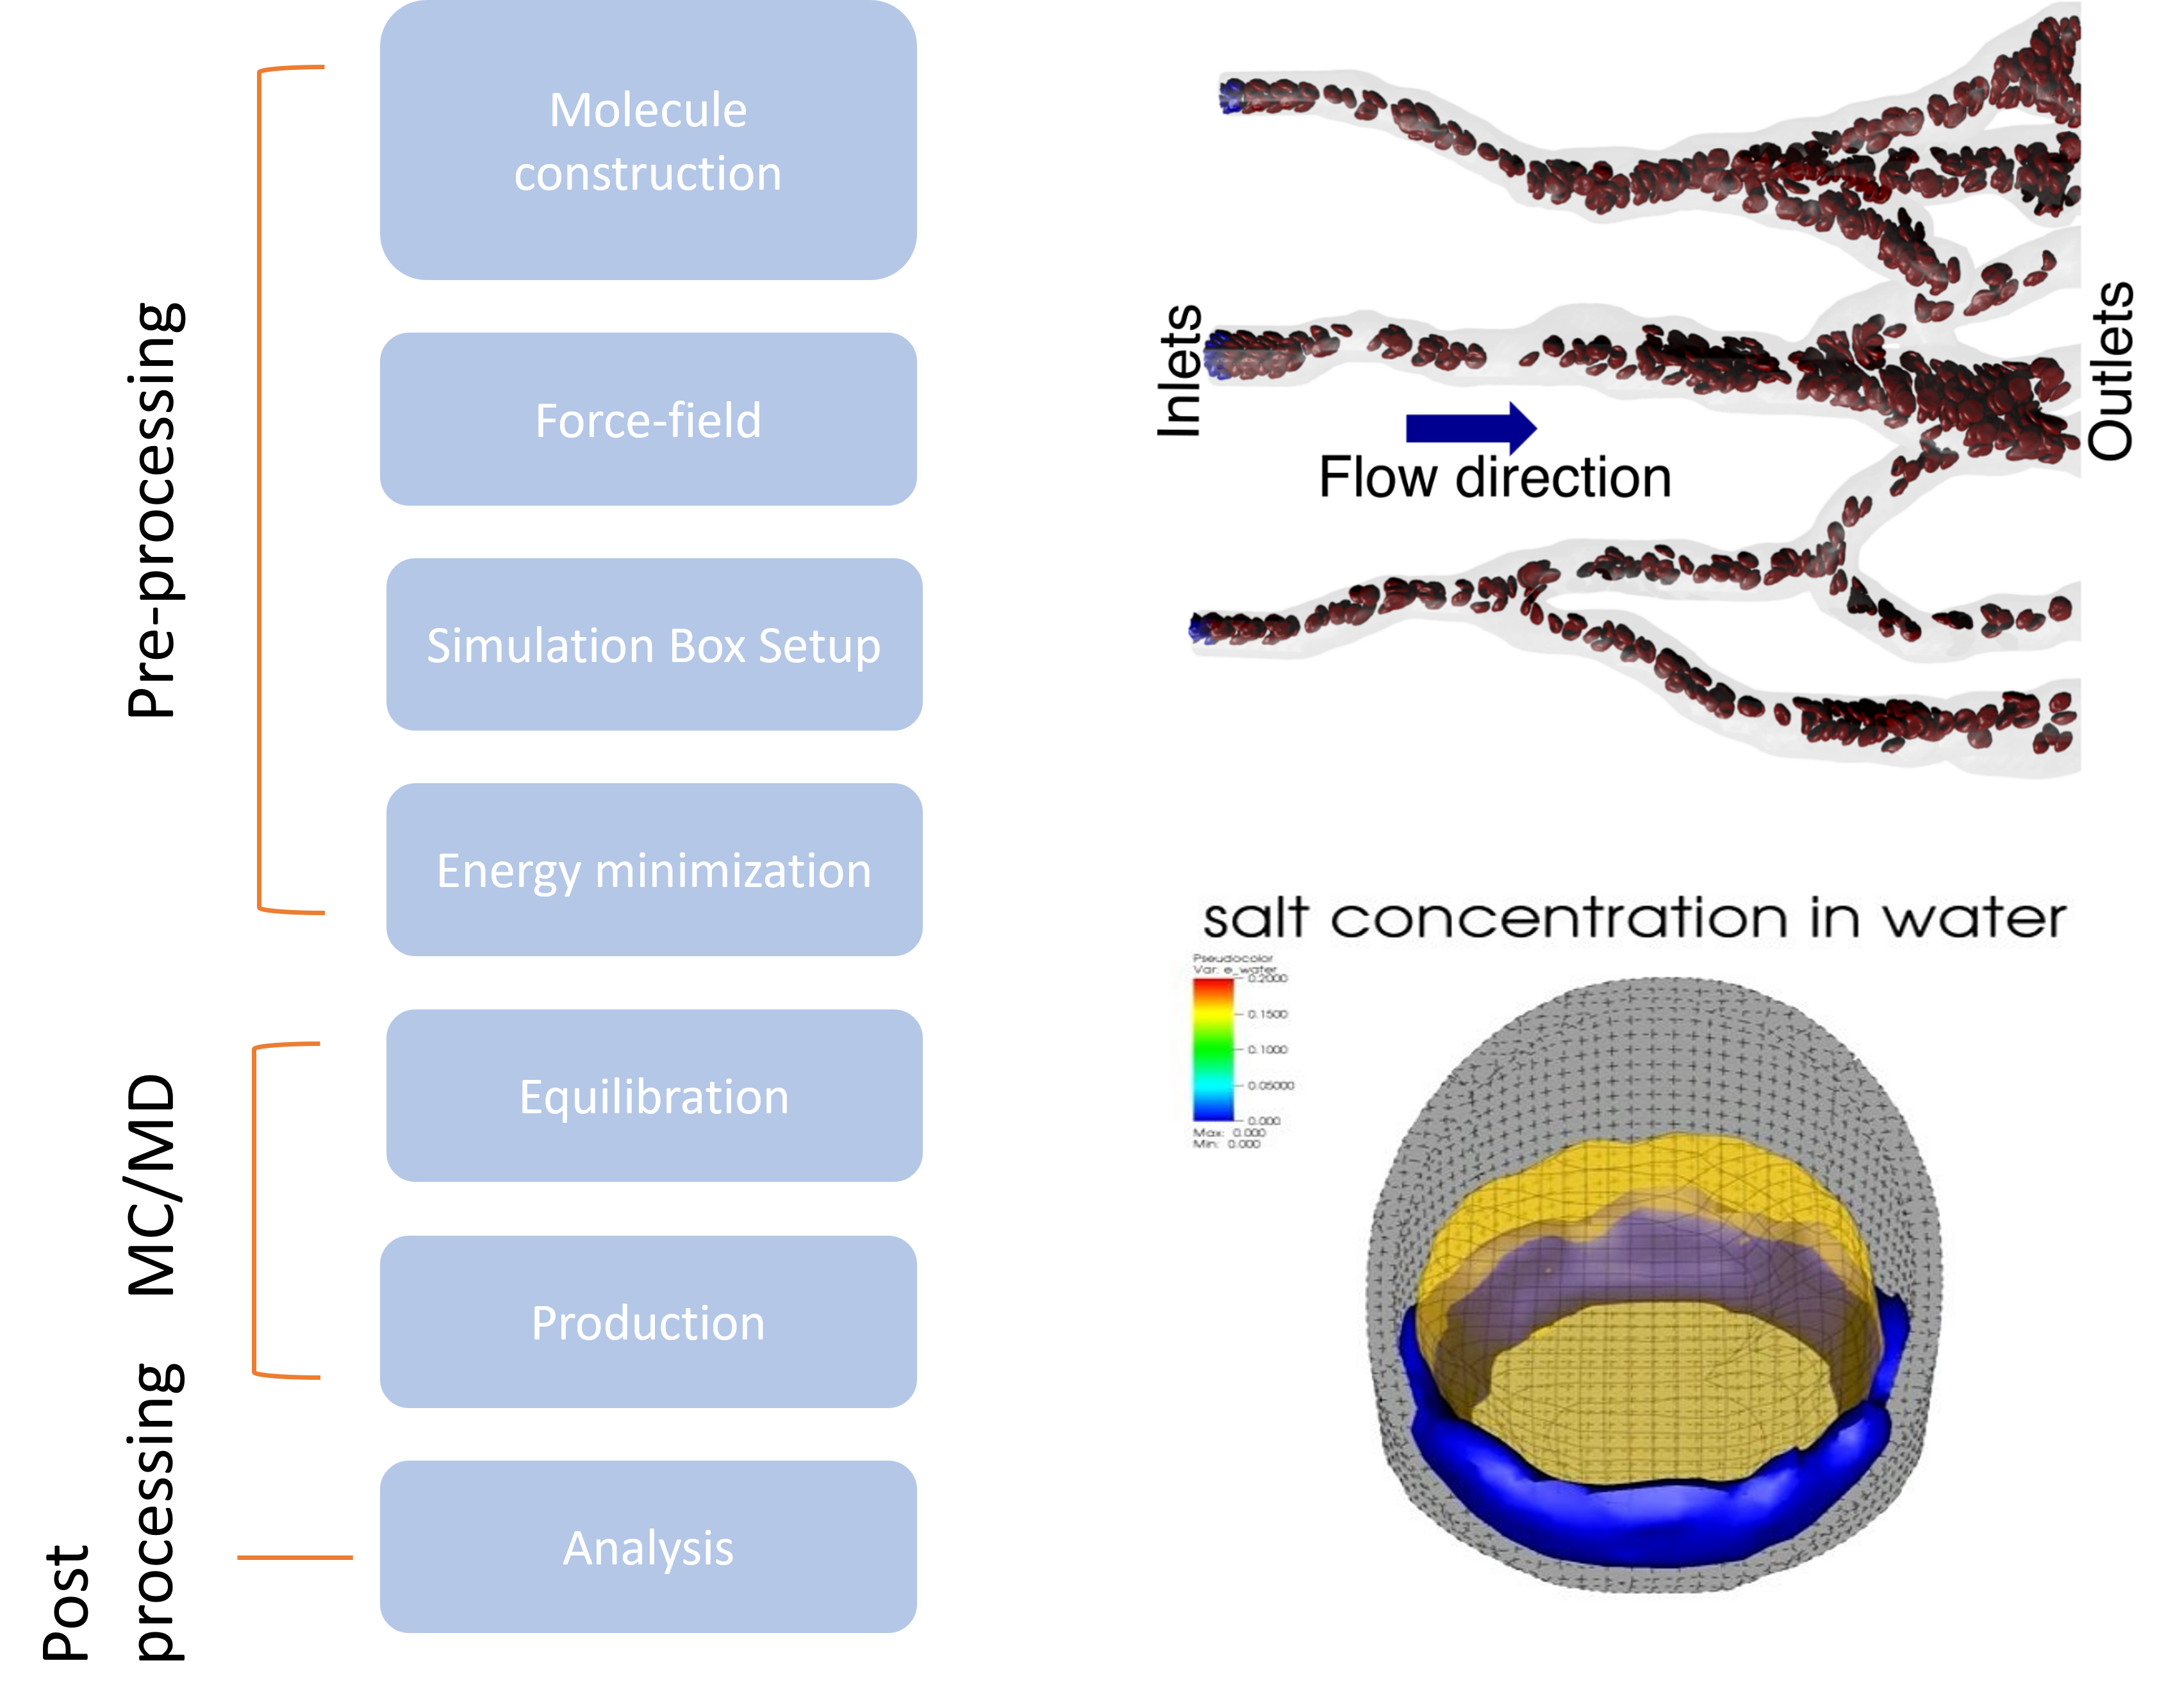
\includegraphics[width=0.7\textwidth]{lammps_flow.png}
  \caption{LAMMPS 模拟流程图}
\end{figure}

\section{函数分析}

\subsection{代码框架}
图 3.1 给出了 LAMMPS 中 eFF 势函数的计算过程, 整个计算包含两次 for 循环,第一层for 循环迭代体系中每个一个粒子,作为计算中的i,第二层循环则遍历迭代每个i 的邻居粒子,其中粒子由邻居列表给出,在确定粒子间距在对应的截断半径内后,开始进行粒子间受力的计算,在计算中由于粒子类型的不同,半径和带电量都会有所差别,并且这里会采用不同的计算方法,之后会给出此轮计算的最终受力,分别累加到 i,j 粒子上。

\subsection{数据结构}
图 3.2 是 LAMMPS 中 eFF 计算中需要的数据结构,大致分类两类,第一类是粒子本身保存的数据,例如粒子坐标,类型,带电量等,这类数据大多是在计算输入文件中直接给出的,第二类则是在计算中体系生成的邻接表相关的信息。


\begin{table}[]
   \centering
  \caption{electron Force Field potential 基本数据结构}
\begin{tabular}{@{}l|l|l@{}}
\toprule
类                      & 数据变量         & 含义                                                                                           \\ \midrule
\multirow{6}{*}{atoms} & coordinate   & \begin{tabular}[c]{@{}l@{}}当前进程所拥有的粒子位置信息, 第一维代表粒子\\ 序号, 第二维分别代表 x,y,z 三维上的位置信息\end{tabular} \\ \cmidrule(l){2-3} 
                       & electricity  & 不同类型和序号粒子的带电量                                                                                \\ \cmidrule(l){2-3} 
                       & force        & \begin{tabular}[c]{@{}l@{}}进程中不同粒子的受力信息, 第一维代表粒子\\ 序号, 第二维分别代表 x,y,z 三维上的受力\end{tabular}     \\ \cmidrule(l){2-3} 
                       & type         & 对应不同粒子的类型信息,例如: 氢原子,电子                                                                       \\ \cmidrule(l){2-3} 
                       & spin         & 对应不同粒子的自旋类型,例如: 原子核,电子                                                                       \\ \cmidrule(l){2-3} 
                       & nlocal       & 当前 MPI 进程所拥有的粒子数                                                                             \\ \midrule
\multirow{4}{*}{lists} & ilist        & 对应粒子的索引位置                                                                                    \\ \cmidrule(l){2-3} 
                       & inum         & 邻接表中 I 粒子数量                                                                                  \\ \cmidrule(l){2-3} 
                       & numneigh     & 邻接表中的每个 I 粒子对应的 J 粒子数量                                                                       \\ \cmidrule(l){2-3} 
                       & firstneigh   & 每个 I 粒子对应的 J 粒子序号                                                                            \\ \midrule
\multirow{2}{*}{pairs} & eatom        & 每个粒子的能量                                                                                      \\ \cmidrule(l){2-3} 
                       & cutsq        & 不同类型粒子直接的截断半径                                                                                \\ \midrule
force                  & newton\_pair & 牛顿第三定律参量标志位                                                                                  \\ \bottomrule
\end{tabular}
\end{table}


\section{主核移植}
申威处理器作为并行处理器,计算的并行实现很大程度上需要依赖从核得高效计算和并行,但主核绝非出于次要的位置。主核自身功能与通用处理器类似,能够执行独立的进程,这就意味着在并行之前,我们可以先将程序移植到主核上,主要目的不仅仅是能够作为计算并行和优化的起点,更主要的是可以将其作为依据,确保计算在移植前和优化后的结果一致。

\begin{algorithm}[h]
  \SetAlgoLined
  \KwIn{$\vec{X}$,Q:整个体系中不同粒子的坐标和带电量\newline
    S,R,T:粒子自旋,波包半径,类型\newline
    L:邻接表\newline
    n:体系中的粒子总数\newline
    $r_{cut}$:截断半径
  }
  \KwOut{$\vec{F}$:粒子受力\newline
    E:体系中的eFF势能
  }

  \For {$i\in[0...n)$}{
      \For {$j\in L_j$}{
        $\vec{r_{ij}} \leftarrow \vec{x_i}-\vec{x_j}$\;
        $ r_{ij}^2 \leftarrow r_{ij}·r_{ij}$\;
        \If {$r_{ij}^2 < r_{cut}^2$}{
          $ dspline_i \leftarrow cutoff(r_{ij})$\;
          \uIf {$S_i = 0 \&\& S_j = 0$}{
            $fpair,ecoul \leftarrow ElecNucNuc(Q,r_{ij})$\;
          }\uElseIf{$S_i = 0 \&\& abs(S_j) = 1$}{
              $fpair,ecoul \leftarrow ElecNucElec(Q,r_{ij})$\;
          }\uElseIf{$abs(S_i = 1) \&\& S_j = 0$}{
            $fpair,ecoul \leftarrow ElecNucElec(Q,r_{ij})$\;
          }\ElseIf{$abs(S_i = 1) \&\& abs(S_j) = 1$}{
            $fpair,ecoul \leftarrow ElecElecElec(Q,r_{ij})$\;
          }
          $fpair \leftarrow fpair·dspline$\;
          $E \leftarrow ecoul·dspline$\;
          $\vec{f} \leftarrow SmallRForce(fpair,\vec{X})$\;
          $\vec{F_i} \leftarrow \vec{F_i}+\vec{f}$\;
          $\vec{F_j} \leftarrow \vec{F_j}+\vec{f}$\;
        }
      }
  }
  \caption{electron Force Field 势函数核心计算}
  \label{algo:algorithm1}
\end{algorithm}



申威处理器主核具有类似于通用处理器的运行流程,这样移植到主核上时程序本身基本可以不做修改。而主要工作就是修改编译环境,其中核心的是替换编译器,设置编译和链接路径,增加对应的编译参数,保证计算的正确性。

\section{eFF 势函数计算在申威处理器上的并行实现}
\subsection{程序移植}
LAMMPS 作为一款分子动力学计算平台,其主要设计模型主要是使用 C++ 语言实现,这不仅在支持众多特性的同时,也使整个模型脉络和层次更加清晰,这当前几乎所有分子动力学平台一致采用的方案。但对于申威处理器来说,却并不是一个优势,反而成为了移植并行的一个障碍。从核编译器无法直接进行C++ 代码的编译,而进行并行和优化的前提正是高效利用从核进行计算。所以实现并行的第一步就是要把热点计算的部分重新以 C 语言实现,并剔除 C++ 中相关的语言特性,诸如类和对象,虚函数等。利用申威处理器的交叉编译来完成编译链接,为此设计了一个用于数据传递的结构体,其中包含了表 K 中的列出的所有计算信息。

除此之外,由于在访问结构体,数组,向量等数据时,不对齐的Load/Store操作会引发不对齐访存异常,主核在收到异常会将指令拆分,但性能会大幅降低,而从核在引发异常后,程序会直接退出。这里有两种解决方法,第一种是在编译时加入-faddress\_align=N 编译选项,保证所有结构体,数组的首地址都以N字节对齐;第二种是在创建数组,结构体时加入\_\_attribute\_\_(aligned(size)) 进行手动对齐。前一种方法采用一种全局配置的方法解决访存对齐的问题,但同时会使编译器对其他无关访存操作的结构体,数组的首地址进行对齐处理,所以我们为了保证访存性能,选择后一种方案进行手动对齐。

\subsection{任务划分}
在进行 eFF 势函数计算中,绝大部分计算都集中在对两体势计算的过程中,也正因为如此对势函数的计算过程需要在从核中进行并行实现,算法核心框架如图 K 所示。整个势函数计算主要由两层迭代构成,外层循环遍历整个体系的粒子,计算规模由体系自身的粒子总量决定,可达千万量级。内层for 循环迭代粒子自身周边的邻居粒子,由邻接表指定,规模与体系内粒子密度和截断半径相关,一般来说在数百左右。

利用从核进行计算并行的关键,就是要对这两层循环进行拆分,由于外层循环规模要明显大于内层循环,所以将外层循环拆分实现从核级并行是最优的方法。但由于分子动力学中牛顿第三定律的引入,导致在更新中心粒子受力的同时,不可避免地需要同时更新邻居粒子的受力情况,这样一来就会加剧计算时的数据依赖和存储空间限制等问题。下面会提出多种并行方案,通过平衡并行粒度,存储空间使用和计算量来找出对于计算 eFF 势函数更合适的并行方案。

\subsection{内层循环并行}
根据对势函数计算的分析,整体计算的并行主要是依赖于对内外层循环的拆分,并均匀分配到从核上。但由于牛顿第三定律的引入,在进行中心粒子的计算时,周围截断半径内的粒子受力信息也一并会更新,这使得在并行时数据依赖成为了一个棘手的问题。

为了解决数据依赖的问题,这里选择了只对内层循环进行拆分,就是对单个粒子的邻居粒子计算进行拆分,并在每个周期对从核分配 N 个粒子对的计算,这样为了保证对于每个从核能够在一个执行周期内时间基本一致。



当每个从核进行 i 粒子与 N 个邻居粒子的粒子对的计算时,由于在这 N 次计算中i 粒子的坐标,电荷量等粒子信息会被多次调用,所以这些信息在计算时会一直保存在从核LDM 中,直到当前粒子计算完成,这就避免了从核频繁访问主存带来的开销。

当每个从核对同一个进行所有邻居粒子的计算时,由于需要同时对i 粒子受力情况等信息进行更新时,就会带来写依赖的问题,不同从核会在进行 N 个粒子对的计算完成之后,进行并发地对i 粒子受力信息的更新,从而引发数据写写依赖的问题。这里选择在计算受力信息完成后不立即更新i 粒子,而是只保留每个从核计算后的增量,并保存在LDM 中,只有当整个粒子与所有邻居粒子的计算完成之后,才进行对受力情况的累加。这里选择0 号从核作为受力信息变化量的接收方,每个从核在累加受力情况之前,需要对从核间进行同步,以此来保证数据的一致性,之后每个从核会逐步将受力信息累加到0 号从核,在最终受力计算完成后,只由 0 号从核完成受力结构的写回,实现整个 i 粒子部分的计算。

除了不同从核在更新i 粒子受力情况时会出现写写依赖,在单个从核完成对i 粒子的计算之后,进行下一个 i 粒子的计算时会出现读写依赖。这是因为上一个粒子的计算结果是由 0 号从核单独写回的,而从核访存需要数百个时钟周期来进行,速度要远低于计算指令的执行速度,就会出现在从核在进行下一个粒子的计算时,上个粒子的结果还没有写回,造成读写依赖。这里需要在每个从核在完成对同一个i 粒子的计算后,等待0 号从核完成粒子信息的写回,进行从核核组内的同步,消除读写数据依赖。还有一个注意的问题就是写回数据的连续性。由于牛顿第三定律的引入,受力等写回信息会被不同从核多次进行更新,这也就要求每次在访存的时候不能只对粒子坐标,带电量等不进行写回的数据读取,还需要读取受力等只写数据,并将此轮计算结果进行累加,保证数据的连续和正确。

\subsection{副本规约方法}
对于内层循环并行方法,将第 i 层粒子与邻居粒子之间的计算实现了并行,在解决局部数据依赖的同时,一定程度上实现了从核级并行。但最大的问题就是每个粒子的邻居粒子数量十分有限,只有不到一千个,这在进行计算划分时从根本上限制了其并行粒度。为了提高计算的并行粒度,副本归约的方法采用对外层循环进行拆分,由于第i 层循环次数与体系规模有关,在体系中计算粒子的数量达到百万乃至千万的量级,并行粒度要远大于内层循环并行的方法。副本归约的方法每次将 N 个第 i 层粒子的计算赋给单个从核,对于 0 号从核计算 0 到第N-1 粒子,第N 到第2N-1 的粒子分给1 号从核,按照这个方法均匀分配了64 个从核之后,剩下的粒子依旧按照上述次序划分,知道所有粒子均划分完成。接下来讨论 N 的取值情况,得到一个合适的 N 值要考虑多方面的因素,在不同计算体系和规模下 N 的取值也可能是不同的。这里给出能够影响 N 取值的因素以及如何平衡 N 的取值。由于要保证一定的从核并行计算粒度,并且在当分配粒子数过少时对于访存会产生更大的开销,但又当 N 值过大的时候,每次所保存在LDM 中的粒子信息又会过大,由于存储空间的限制,又无法保证大规模计算的进行,并且在最后一轮的计算中,从核间计算的分配又会更加不均匀,反过来影响计算性能。

在副本归约方法中,数据写依赖的问题会变得更加严峻,因为对外层粒子循环进行拆分会对中心粒子和邻居粒子同时进行多次更新,为了解决存在粒子被多个从核同时更新造成写写依赖的问题,每个从核LDM 都会开辟一份单独的空间,在从核计算完受力等信息后,不直接对粒子进行写回,而是将结果写到临时空间内,等到从核此轮计算全部结束后,由0 号从核完成计算结果的累加,并单独写回主存。

这种方法虽然能够提高并行性,但由于需要为 64 个从核在 LDM 中单独开辟一个副本,这对存储空间来说是一个极大的消耗,在计算规模过大的时候,这无疑是不可接受的。下一章会介绍一种通过平衡计算量,并保证从核计算并行度和计算规模的方法。
